\documentclass[12pt]{report}
\usepackage[a4paper,top=3cm,bottom=2cm, left=3cm, right=2cm]{geometry}
\usepackage[utf8]{inputenc}
\usepackage{listings}
\usepackage{graphicx}
\usepackage{mathdots}
\usepackage{tikz}
\usepackage{booktabs}
\usepackage{pgffor} 
\usepackage{float}
\usepackage{graphics} 
\usepackage{fancyhdr}
\usepackage[square, sort, numbers]{natbib}
\usepackage{color}
\usepackage{indentfirst}
\usepackage{epigraph}
\usepackage{ragged2e}
\usepackage{blindtext}
\usepackage{amsmath,amsthm,amssymb}
\usepackage{tabto}
\usepackage{pgfplots}
\usepackage{changepage}
\usepackage{subcaption}
\usepackage{fancyvrb}
\usepackage{caption}
\usepackage{minted}
\usepackage{placeins} % put this in your pre-amble
\usepackage{flafter}  % put this in your pre-amble

\usetikzlibrary{patterns}
\usetikzlibrary{arrows.meta}

\graphicspath{{images/}}

\definecolor{mycolor}{RGB}{30,75,180}
\definecolor{mycolor2}{RGB}{40,75,90}
\definecolor{red}{RGB}{200,0,0}
\usepackage[colorlinks = true,
            linkcolor = mycolor,
            urlcolor  = mycolor,
            citecolor = mycolor,
            anchorcolor = mycolor]{hyperref}

\usepackage[hypcap=true,font={small,it}]{caption}
\usepackage{pdfpages}
\usetikzlibrary{calc}

\captionsetup{belowskip=2pt,aboveskip=2pt}

\bibliographystyle{abstract}

\renewcommand{\chaptername}{}

\renewcommand{\figureautorefname}{figure} % lower case default ref
\renewcommand{\tableautorefname}{table} % lower case default ref
\let\oldchapter\chapter% Store \section in \oldsection
\renewcommand{\chapter}{\cleardoublepage\oldchapter}% Prepend new \section with \cleardoublepage

\newcommand{\latex}{\LaTeX\xspace}
\newcommand{\mcite}[1]{\textcolor{mycolor}{\citeauthor{#1} (\citeyear{#1})}}
\newcommand{\hcite}[1]{(\textcolor{mycolor}{\citeauthor{#1}, \citeyear{#1}})}
\newcommand{\defi}[1]{\textbf{#1}}
\newcommand{\naming}[1]{\textbf{#1}}
\newcommand{\todo}[1]{\textbf{\color{red} TODO: #1}}
\newcommand{\gam}[2]{\mbox{$\{#1\:|\:#2\}$}}
\newcommand{\Gm}[1]{\mbox{$G#1$}}
\newcommand{\Hm}{\mbox{$H\,$}}

\definecolor{purple2}{RGB}{218,112,214}

\pgfplotsset{style thermograph/.style={
		axis x line*=none, axis y line*=none,
		axis line style={draw=none},
		y label style={rotate=-90,at={(current axis.north west)}, right=5mm},
		ylabel = \textbf{t},
	}
}
\lstset{
	columns=fullflexible,
	mathescape=true,
	numbers=none,
	stepnumber=1,
	morekeywords={return, if, else,  while, vector, using, include, class,
		true, false, function, or, public, private},
	xleftmargin=4.0ex,
	tabsize=4,
	frame = single
}

\makeatletter
\renewcommand{\thesection}{%
	\ifnum\c@chapter<1 \@arabic\c@section
	\else \thechapter.\@arabic\c@section
	\fi
}
\makeatother

%----------------------------------------------------------------------------------------------------%

%--------------------------------------------- DOCUMENT ---------------------------------------------%
\begin{document}
	\newpage
    \begin{titlepage}
\begin{figure}[H]
    \hspace*{-1.0cm}
    \vspace*{-0.5cm}
    
\includegraphics[scale=1]{images/logo_rit.jpg}\\
\end{figure}

\begin{center}
    \vspace*{2cm}
    
    {\LARGE \textbf{Proposal for Conveyor Sorter System}}
    
    \vspace{0.5cm}
    \textbf{Purpose, environment, configuration, devices and safety measures}
    
	\vspace{1cm}
	 by
    \vspace{1cm}
    
   Matheus Tararam de Laurentys
\end{center}

\vspace{1cm}

\begin{center}   
	{\large Project 1 Report \\ 
		MFET0450 - Automation Control Systems} \\
	\vspace{0.5cm}
	Directed to: Prefessor Michael Slifka \\
	
\end{center}

\vspace{1cm}

\begin{center}
	Report submitted in partial fulfillment of the\\
	requirements for project 1

	\vspace{1.0cm}
	at
	\vspace{1cm}
	
	Rochester Institute of Technology \\
	Department of Manufacturing and Mechanical Engineering Technology \\
	October 2021
\end{center}

\end{titlepage}

	\section{Executive Summary}
    The operation of filling bottles, from those of drinkable waters to containers of washing machine detergent, is highly automated. The high volume and low production cost requirements of these products make automation the only viable option. This report features a system capable of operating with different types of containers and varied liquid materials. The report also dives deep into a program that simulates the production line of bottled liquids. With some adaptations the program can be used to operate on the physical implementation of the system.

The system uses two feeders, one for bottles and one for liquids. When operating, the bottles are moved into a container and get rinsed, filled and caped. Finally the bottles of the same type and liquid, grouped together, are made available to packaging. To operate, the system uses a PLC program that verifies the count of bottles in the feeder to coordinate with moving of products to the conveyor and verifies volume of liquid available to coordinate with filling of bottles.

Other than the two feeders, the system requires a set of colored button devices, a bottle filling machine, a bottle conveyor and the PLC itself. The PLC used is Rockwell's model 5069-L306ER, with models 5069-IB6F and 5069-OB16 as input and output modules. The simulation is implemented in Ladder Logic using Studio 5000.

    \newpage
   
    \section{Full System Description} 
    A common process that requires speed and precision is taking a collection of products, boxes, letters or parts, and breaking it into a set of collections that are related in some way. The sorting conveyor described in this text will take a collection of elements and break it into three other collections based on their sizes. Such a system has many areas of application but, to name one, consider a factory that produces a variety of products of different sizes. At some point the total production will need to be sorted and the conveyor sorting system ("System") is an option to accomplish that.

The System is recommended because it handles high production volumes, but also small ones, faster and in less space than having a team of employees would. The System also has very high accuracy and potentially costs less than maintaining a team to do the same job. In addition, the system is potentially safer to employees and machines than having materials handled manually. Overall, the System will give companies higher revenue.

The System is built to be incorporated to pre-existing production lines but it is also able to operate by itself. It can be installed and operated in common work areas as it will not incur any significant risk to personnel. However, it can be used in fully automated areas as it does not require any human interaction. See the following image.

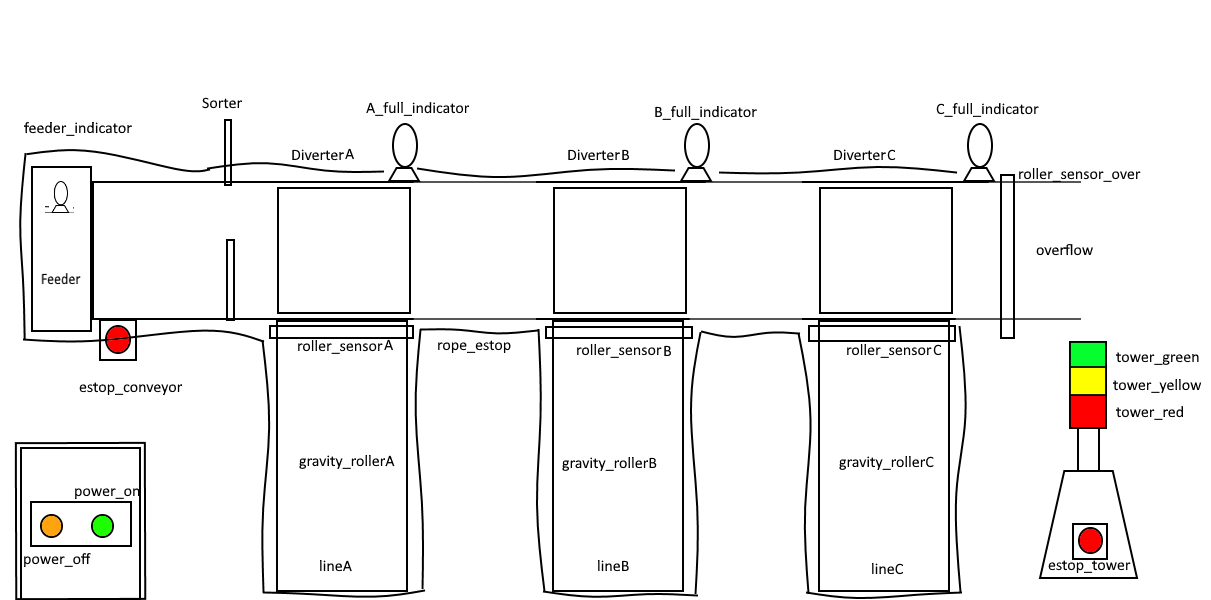
\includegraphics[scale=0.5]{../external/system_graphics_full.png}

Products will flow from the feeder, down to the belt and be sorted and moved, if possible, to their respective lines. If it is not possible to move to the designated area, the conveyor will transport the product to an overflow area. When shutting down or recovering from an emergency stop or power loss, the system will empty the conveyor by moving its products to the same overflow area.

When the feeder is filled with 12 products it will light an indicator light that lets the operator know the system can start running. If the feeder is not full, the system will not run. However, in order to successfully to startup, all emergency stops must also be reset in case they were activated. The first action taken when booting the system red lights will power on and horns will ring. 

After a delay, the system verifies, through internal PLC retentive counters, if it can power the main conveyor or if it should run a recover module. This decision is solely based on the count of products in the conveyor. If there are counter they will be moved to an overflow area. After startup the feeder will feed products at a constant rate until it goes empty. There are indicator lights for when the feeder becomes empty.

The products fed to the conveyor pass by an object detection and sizing sensor that will decide to which line is should go though. After that decision is made the PLC will coordinate the position of the belt diverters so that the products reaches the correct destination. The size is not the only factor in that decision, because if a line is full the PLC program will not allow the product to be moved there and will sent it to the overflow area instead.

A line is considered full either if its collection point capacity is reached or if some predefined total value of products is reached. Those predetermined values for the featured system are 36 for line A, 24 for line B and 18 for line C. The collection point capacity is also set to 8 and 6 for lines A and C, respectively, and unbounded for line B. When wither collection point is full, an indicator light will turn on the tower lights.

The internal counter that is used to decide if the main system can startup when the star push button is pressed works via sensors placed between the rollers of the lines and the overflow area. The count of products in the conveyor is the difference between the amount of projects that were moved from the feeder into the conveyor and the sum of the products that went through either of the four possible destinations.


Finally, when shutting down, normally, the system will make the same conveyor count verification and move of products done in the recovery module. That guarantees it can start safely in the next system startup but also makes sure no products is left behind inside the system, possibly unreachable. 

The final part of the system is the way it handles emergency stop. The current state of the implemented simulation will stop both the main routine and the recovery module immediately. While that is good, it could also trigger breaks on the conveyor instead of letting the inertia take effect. That is one point of improvement that will be discussed by the end of the proposal.











    
    \section{Logic Flow Chart}
    The flow and logic of the System that is implemented in the form of a PLC program. This flow simulates the behavior of the proposed sorting conveyor.

\hspace{-3cm}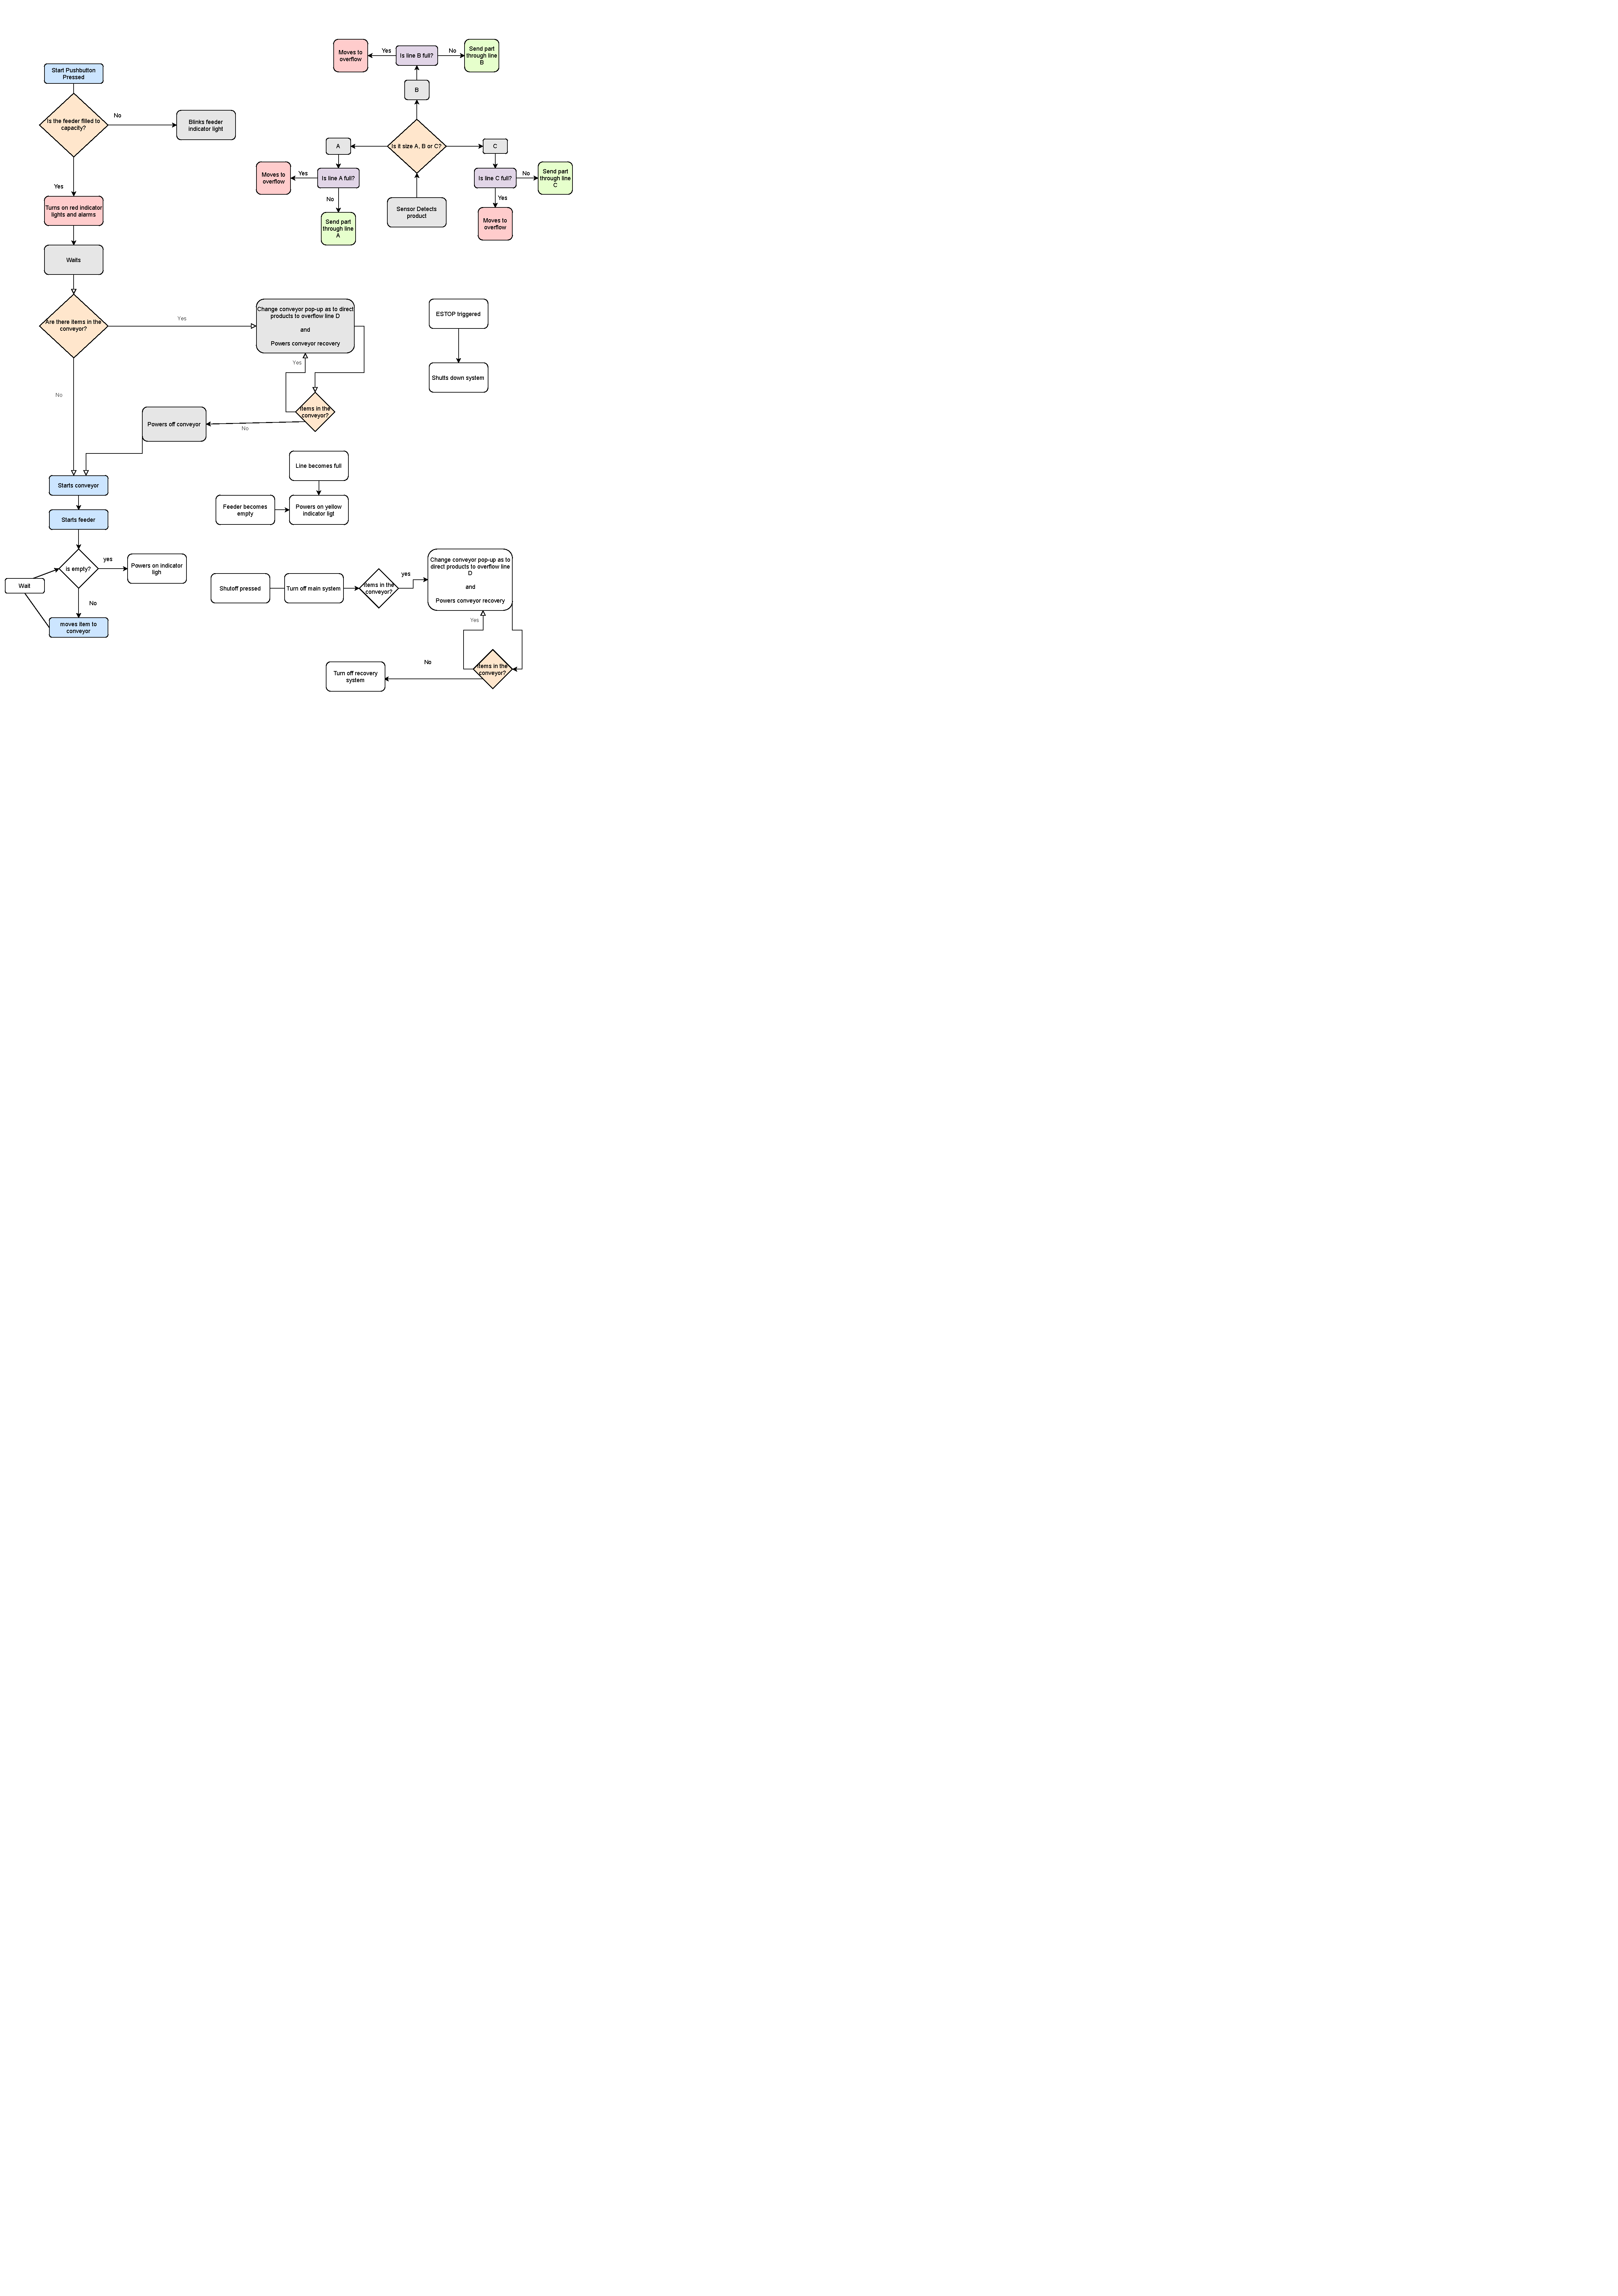
\includegraphics[scale=0.6]{external/logic.pdf}

    \section{Development Spreadsheet}
    \hspace{-1cm}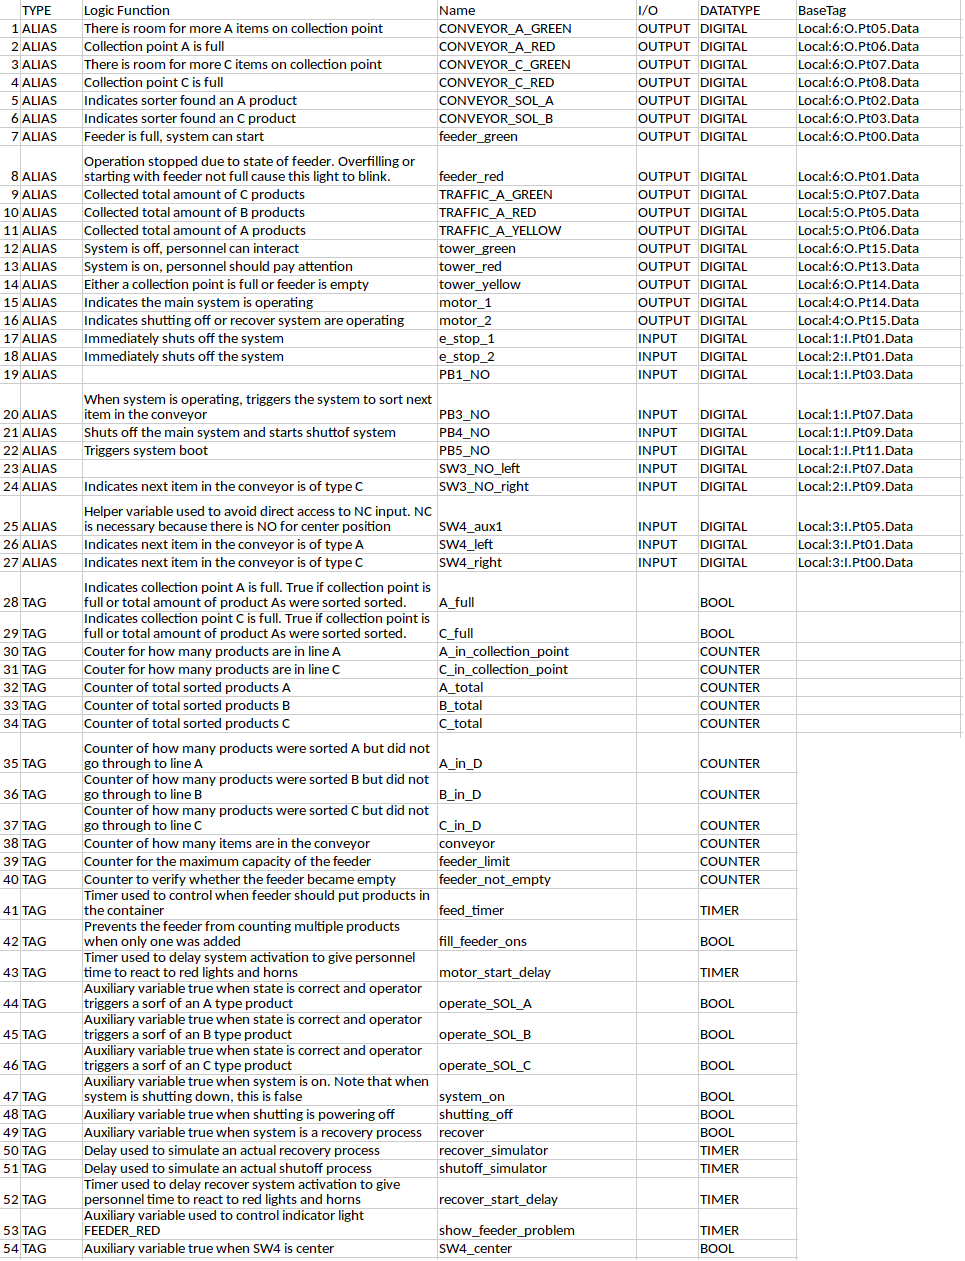
\includegraphics[scale=0.65]{../external/dev_spr.png}
    
    \section{PLC definition and specification}
    \subsection*{Components}

\hspace{-2cm}
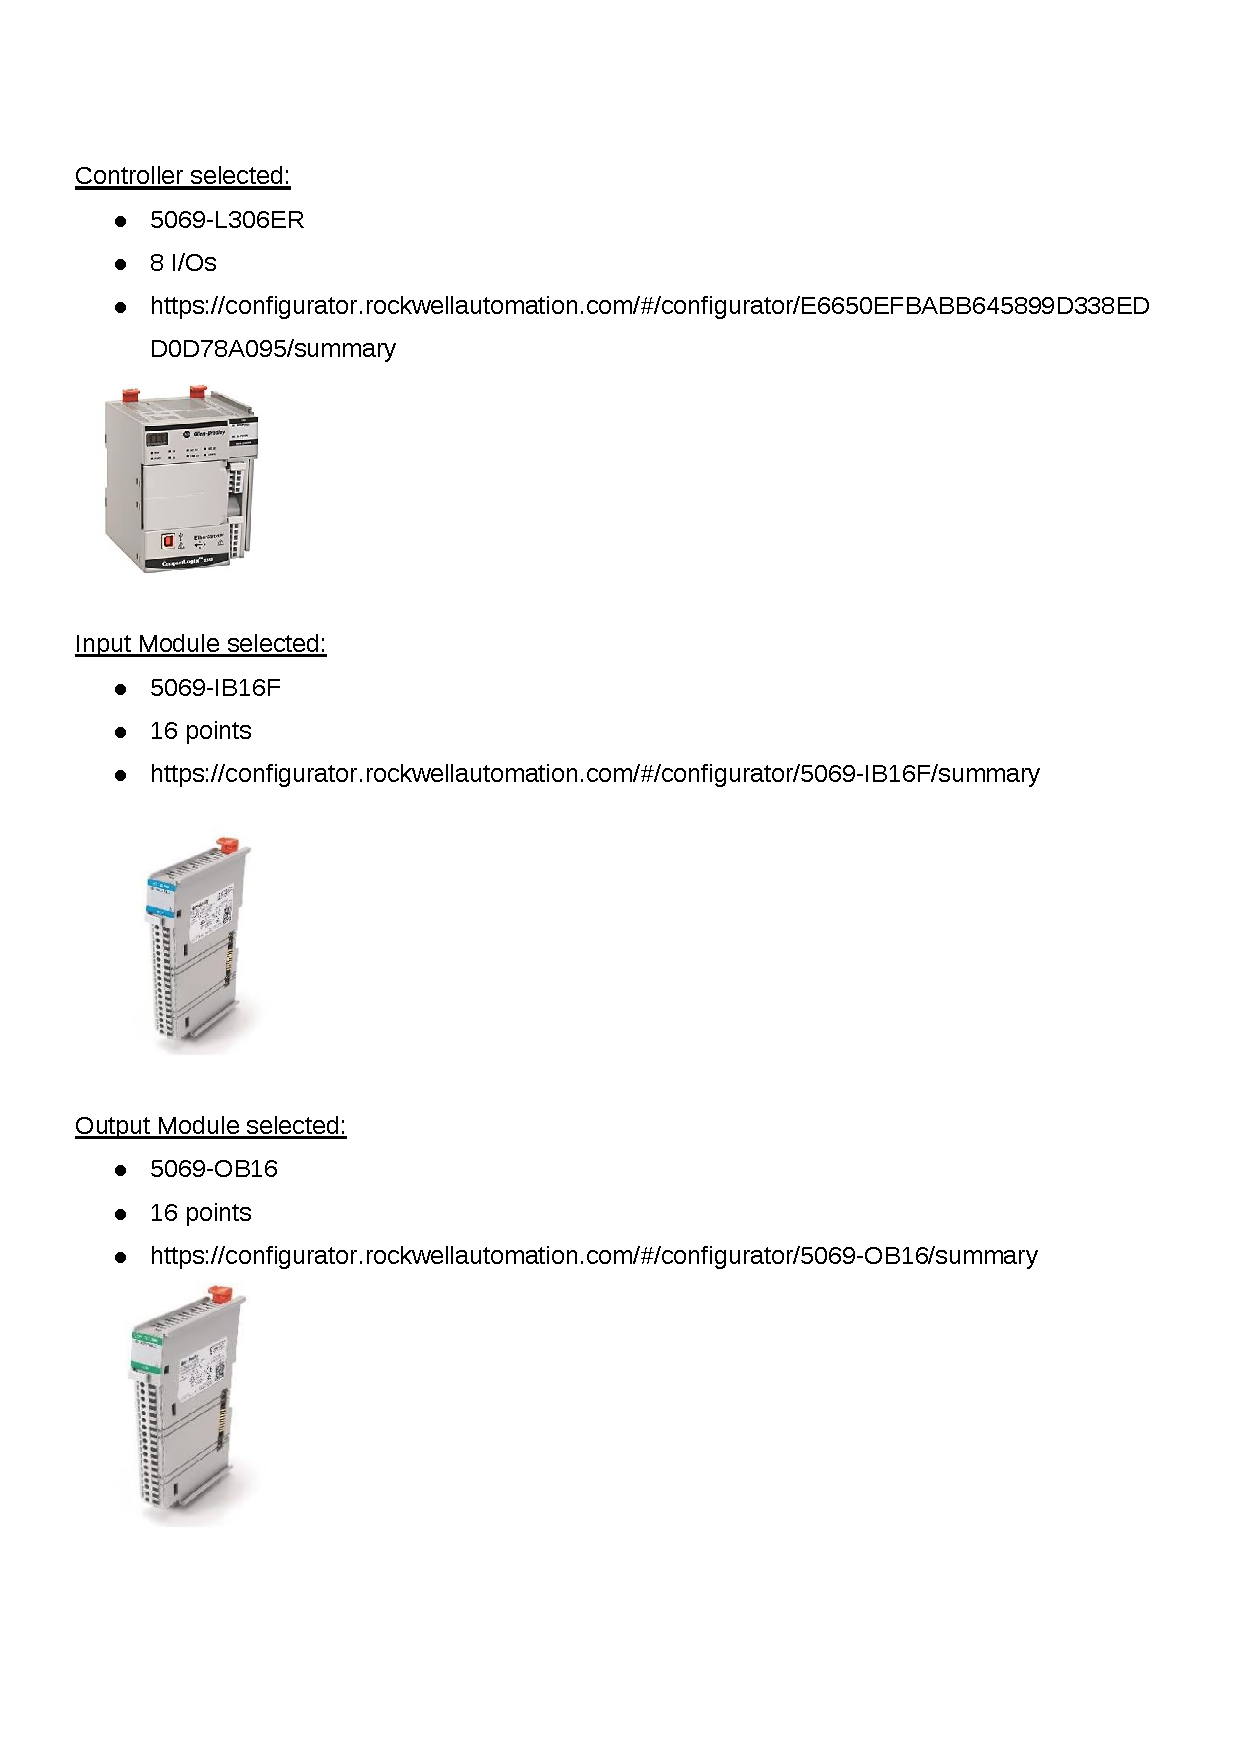
\includegraphics[scale=0.7]{external/plc3.pdf}

\subsection*{Connections}

Find in the table below a possible way to connect the devices listed to the PLC points. Not that only one input and output module are required.

\vspace{1cm}
\hspace{-3cm}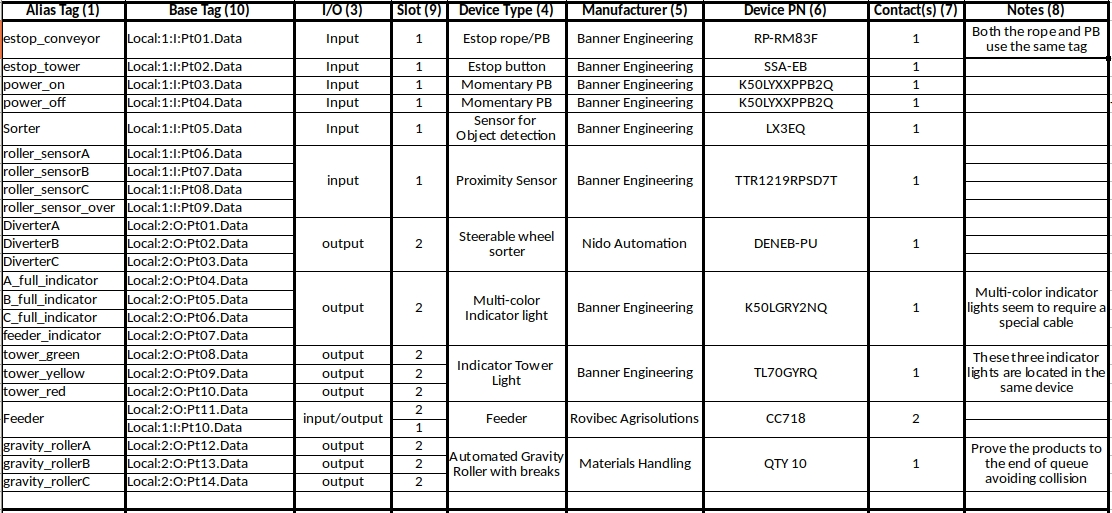
\includegraphics[scale=0.67]{../external/planning.jpeg}
    
    \section{Specification of input and output devices}
    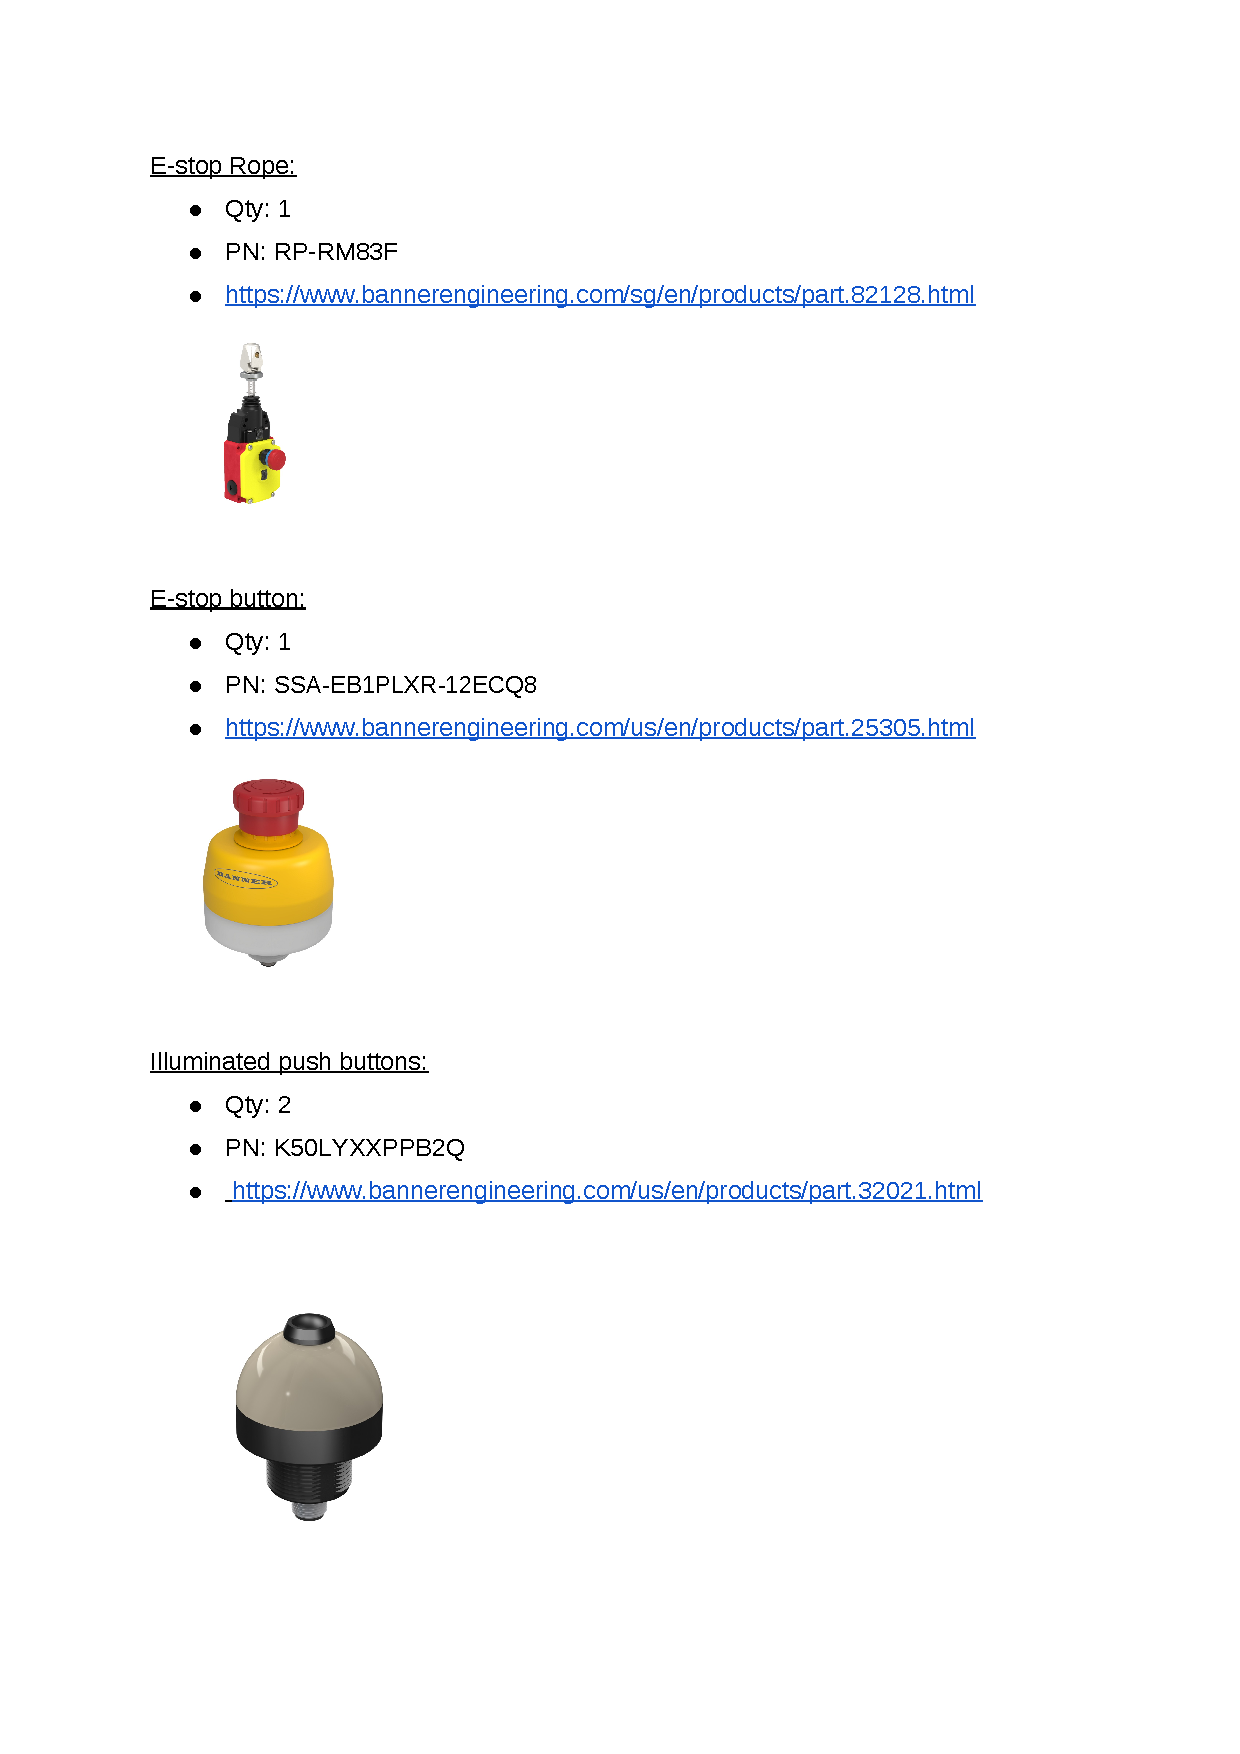
\includepdf[pages=-,pagecommand={}]{external/devices.pdf}
    
    \section{Logic of the system}
    Find the code for the simulation system in the next few pages.

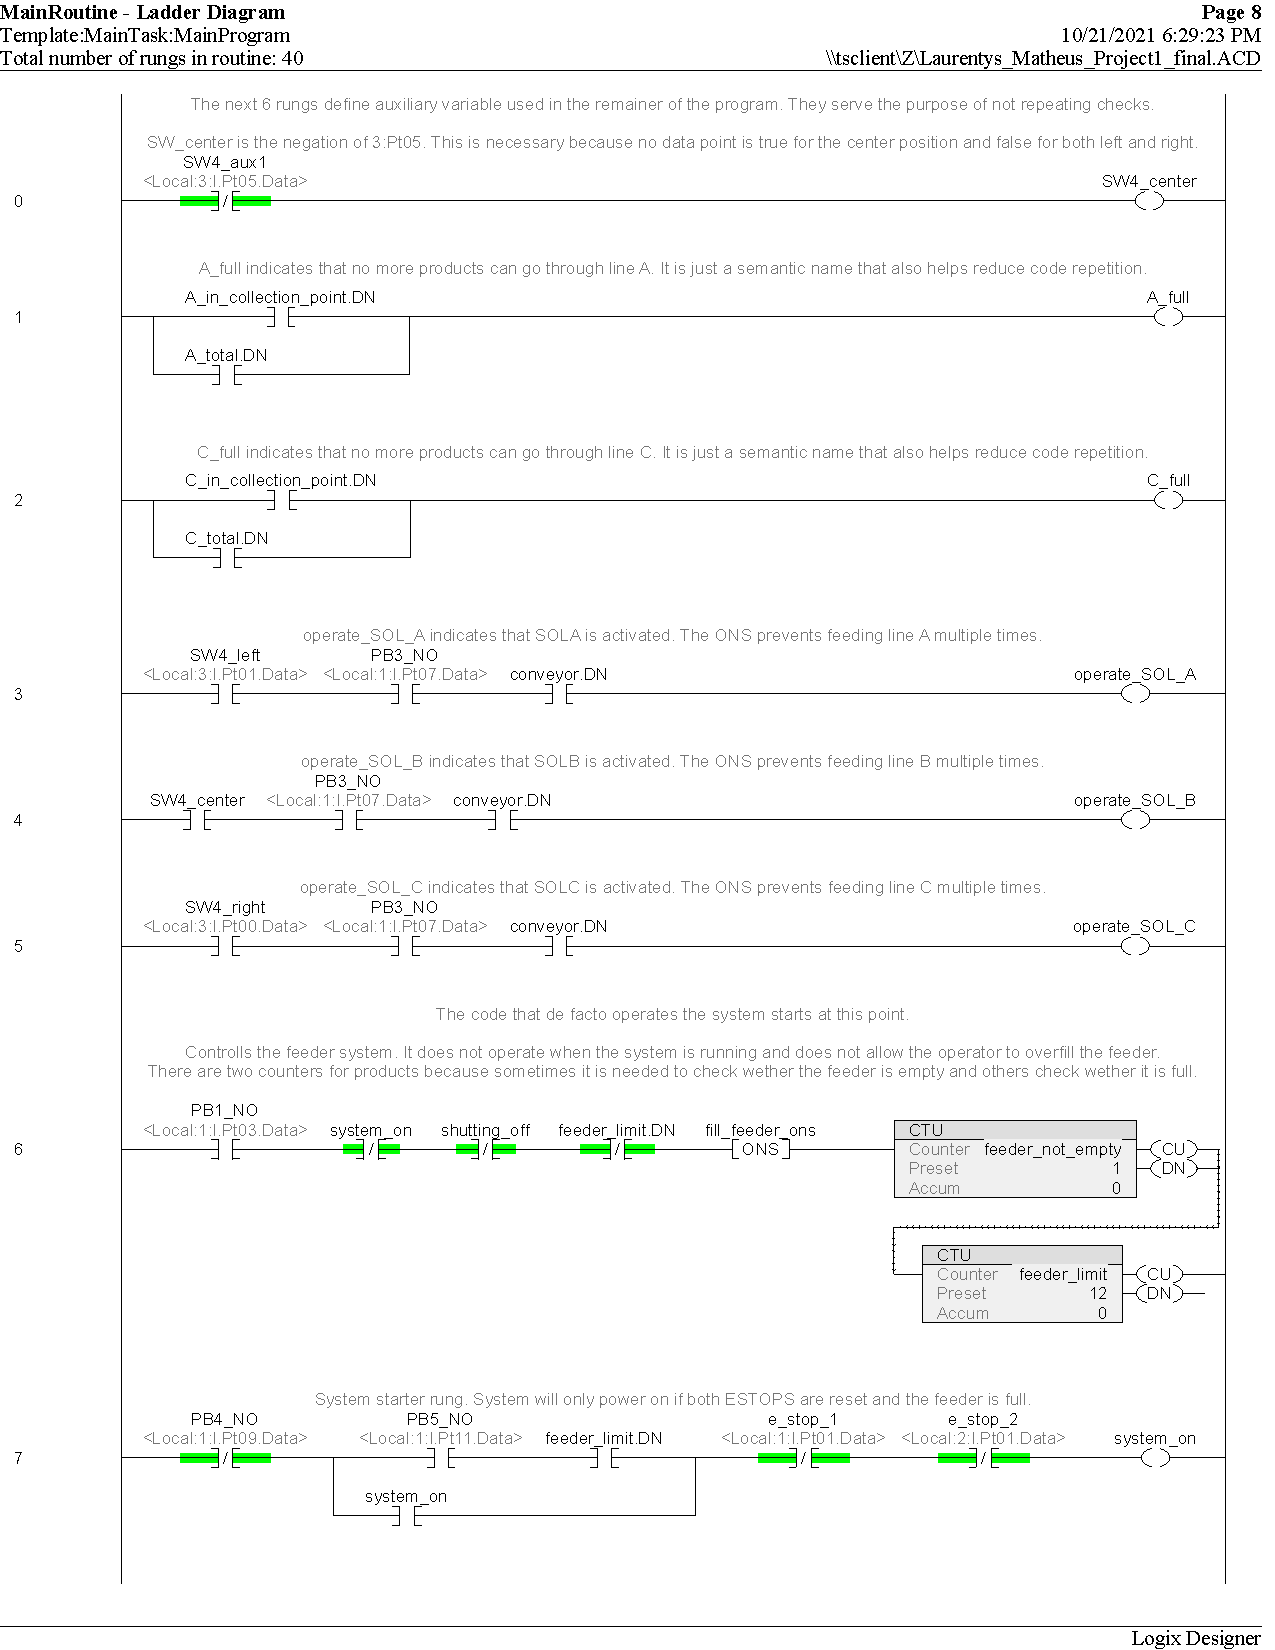
\includepdf[pages=-,pagecommand={}]{external/code.pdf}
    
    \section{Startup Configuration}
    The first requirement for system startup is that emergency stops are reset to their original position. This is a common and necessary procedure. Another requirement to power on the system is having the both the bottles and the liquid feeders with some amount of product.They do not have to be full, but need to be fed to a predefined capacity.

The last requirement is the conveyor to be full. This is a necessity because system supports different types of bottles. If the feeder is fed with a different type of bottle than those in the bottle conveyor, then there would be a big a problem, possibly big, with the output of the system. Once there is a reset, like with a power loss, the system will recover to a safe state by moving everything from the conveyor to a designated overflow area. The same happens when the system is shut off normally: moves shutting off power to the conveyor, objects are, once again, moved to an overflow area.
    
    \section{Potential System Issues}
    The System as implemented in the simulation and described section 2 will resist some errors resulting prom emergency stops and power loss. The current state of the system, however, is not safe for all scenarios, including resistance to personnel mistakes and parts failure. This section brings some of them into light.

Due to the high speed, the bottle conveyor should be kept in a restricted area when operating. Although there is an E-Stop rope around the conveyor, since there are no proximity sensors the speed might be high enough to cause damage to personnel in the restricted area before the E-Stop is actuated. However, this injuries are not major nor fatal, and by making the zone where the System is installed restricted, the accidents will be rare.

If it is impossible to restrict the area where the feeders and fillers are installed, then physical barriers should be added is all reachable parts. In this cases, using proximity sensors is a good addition to system safety. For example, if the part holding the bottles fails, a bottle will fall in a very high speed. If it is in an accessible area and there are no barriers, it might hurt personnel.

Additionally, the system does not take into account misuse of the equipment. As from the PLC program, the packaging points cannot be accessed when the machine is on. packaging is only allowed when conveyor power is off because there is a risk of having other products coming down from the conveyor in high speed. However, since there are no physical blocks that becomes a risk in the physical implementation.

The last featured problem is with material handling and monitoring parts failure. If the liquid feeder fails and does not detect it is out of liquid, the system will continue running normally. While not a risk to personnel, the result would be packaged empty bottles, which is a big problem. The problem is there are no feedback sensors. The system only uses timers and trusts every subsystem works all the time. This is not realistic but is a decision taken to avoid unnecessary complication in the earlier stages of development. If moving to a physical scenario, feedback sensors would be necessary to monitor the system.
    
    \appendix
    \chapter{Specifications Sheet}
    Find specifications sheet starting on the next page.

\includepdf[pages=-,pagecommand={}]{external/final_specs.pdf}
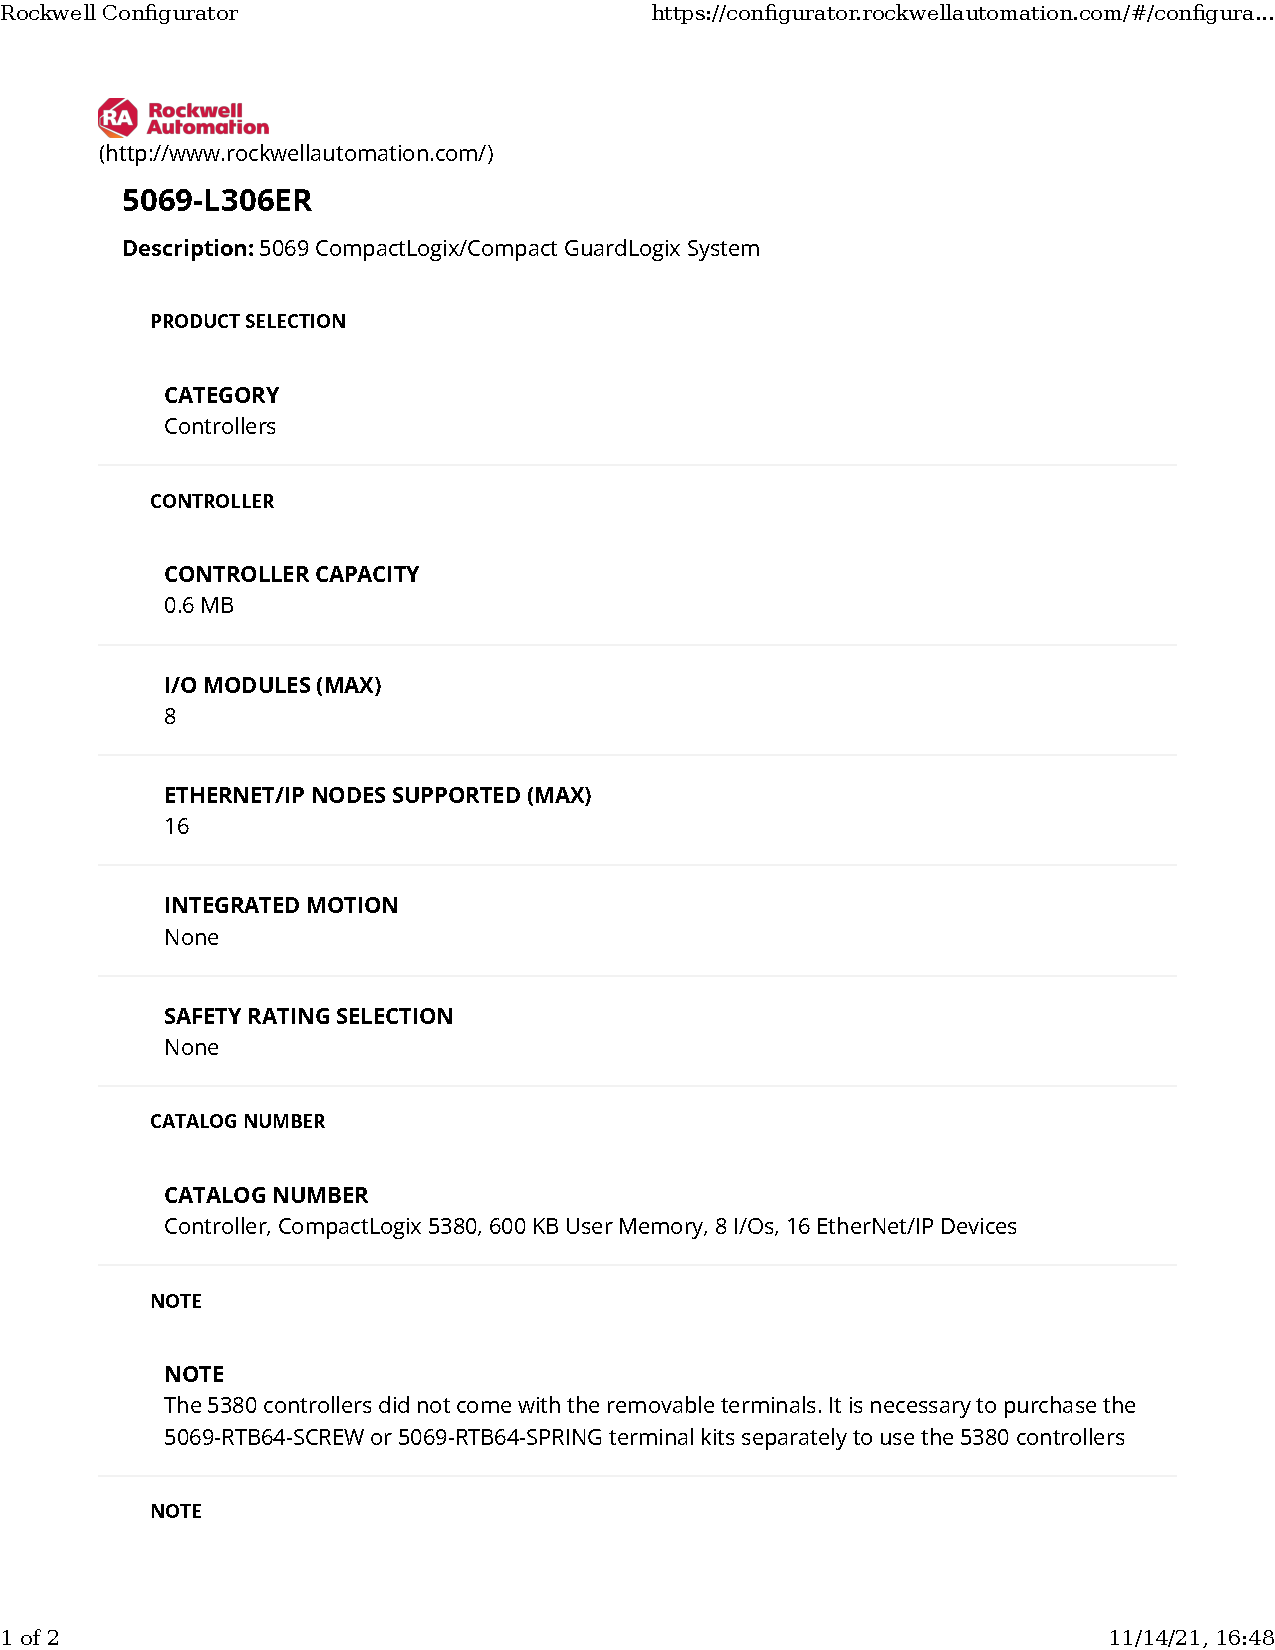
\includepdf[pages=-,pagecommand={}]{external/controller.pdf}
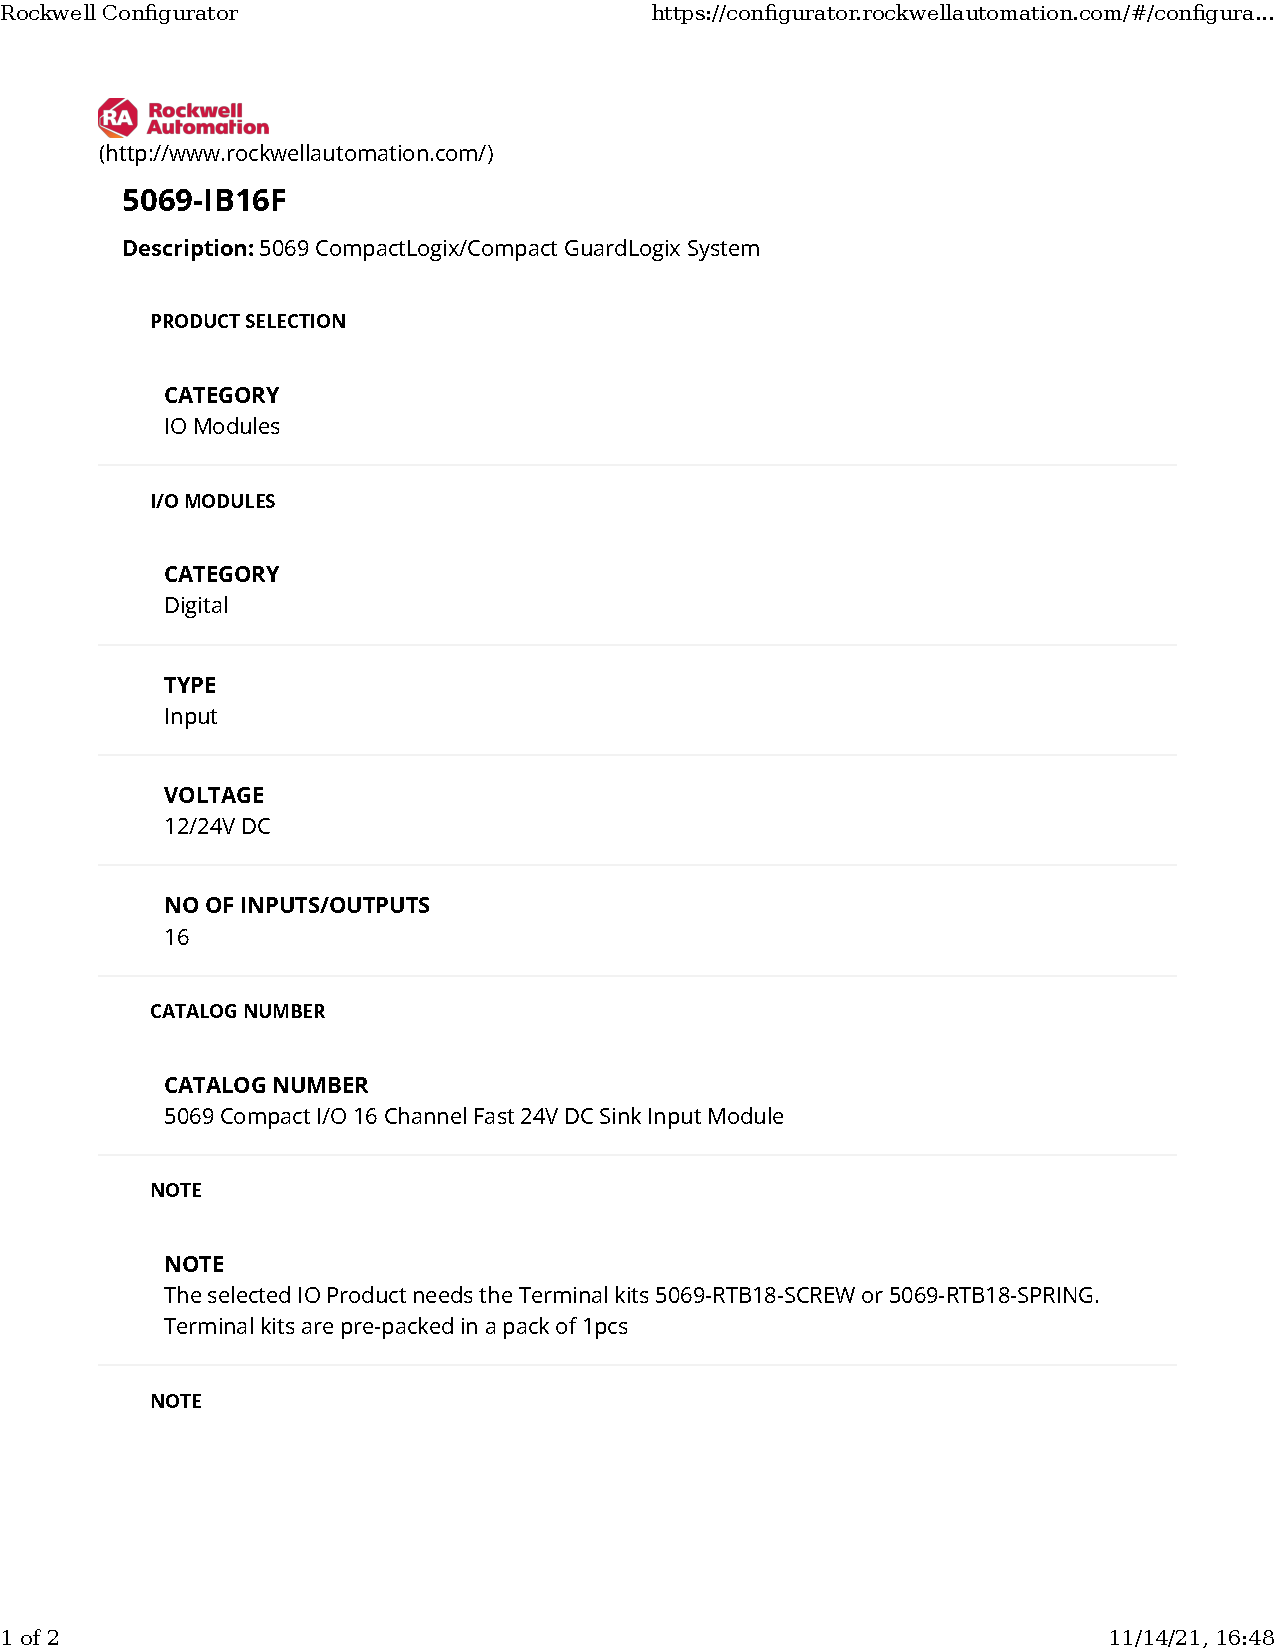
\includepdf[pages=-,pagecommand={}]{external/input.pdf}
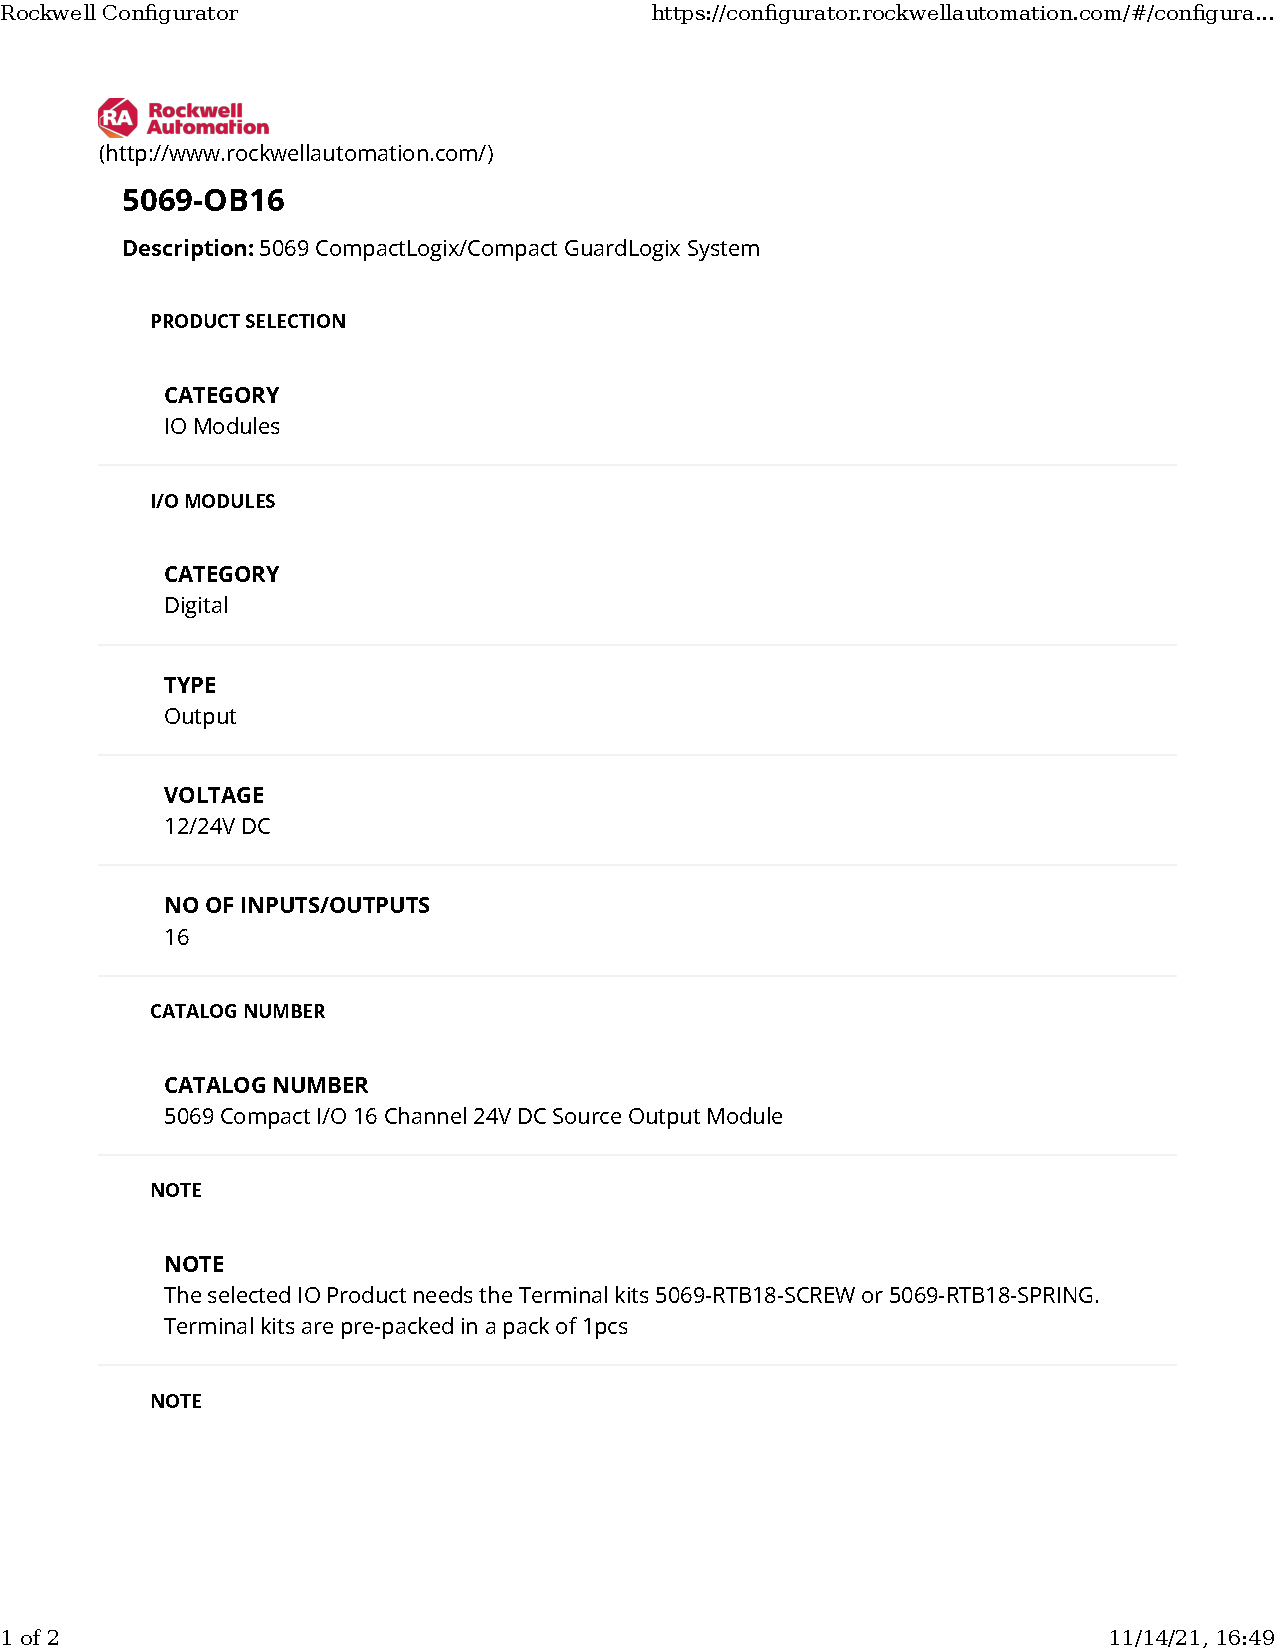
\includepdf[pages=-,pagecommand={}]{external/output.pdf}
    

\end{document}
%----------------------------------------------------------------------------------------------------%
